\section{Synthetic Experiments}
% Generated from frozen experiment artifacts; do not edit.
\newcommand{\ExpOneOuterFolds}{108}
\newcommand{\ExpOneBinaryFeasible}{40}
\newcommand{\ExpOneRegressionFeasible}{16}
\newcommand{\ExpOneNullMin}{3}
\newcommand{\ExpOneNullMax}{13}
\newcommand{\ExpOneAdditiveCoerror}{0.899}
\newcommand{\ExpOneAdditiveForest}{0.784}
\newcommand{\ExpOneAdditiveCatboost}{0.764}
\newcommand{\ExpOneAucGain}{0.0107}

Experiment 001 evaluated nine known mechanisms for each of binary classification
and regression: additive, redundant, correlated blocks, sparse, dominant, XOR,
four-way parity, mixed, and null. Fixed settings were $N=600$, $M=40$, $B=100$,
$K=8$, feature fraction $0.1$, tree depth 3, minimum leaf size 5, two generation
seeds, three outer folds, and three OOF folds. This produced
\ExpOneOuterFolds{} paired outer evaluations. Forest and boosting baselines use
static configurations; search compute, final capacity, and inference budgets
are measured but unmatched.

\begin{table}[t]
\centering\small
\begin{tabular}{lrrrrrrr}
\toprule
Regime & RS & Top & AbsCorr & CoErr & CoErr-all & RF & CatBoost \\
\midrule
additive & 0.655 & 0.689 & 0.701 & 0.693 & 0.693 & 0.809 & 0.794 \\
correlated\_blocks & 0.805 & 0.775 & 0.822 & 0.804 & 0.804 & 0.842 & 0.849 \\
dominant & 0.752 & 0.875$^{\dagger}$ & 0.867$^{\dagger}$ & 0.872$^{\dagger}$ & 0.872 & 0.869 & 0.886 \\
mixed & 0.588 & 0.662 & 0.672 & 0.666 & 0.666 & 0.705 & 0.746 \\
null & 0.506 & 0.527$^{\dagger}$ & 0.535$^{\dagger}$ & 0.509$^{\dagger}$ & 0.529 & 0.500 & 0.522 \\
parity & 0.528 & -- & -- & -- & 0.503 & 0.502 & 0.500 \\
redundant & 0.826 & 0.805 & 0.840 & 0.827 & 0.827 & 0.868 & 0.872 \\
sparse & 0.645 & 0.778 & 0.820 & 0.815 & 0.815 & 0.849 & 0.868 \\
xor & 0.483 & 0.478$^{\dagger}$ & 0.481$^{\dagger}$ & 0.494$^{\dagger}$ & 0.495 & 0.605 & 0.838 \\
\bottomrule
\end{tabular}
\caption{exp\_001\_mechanisms\_v1: binary, auroc. Means over completed outer folds and seeds. --: fixed-K infeasible in every split; $\dagger$: partial feasibility. Full coverage is stored separately. Static baselines, unmatched compute; development only.}
\end{table}

\begin{table}[t]
\centering\small
\begin{tabular}{lrrrrrrr}
\toprule
Regime & RS & Top & AbsCorr & CoErr & CoErr-all & RF & CatBoost \\
\midrule
additive & 0.933 & -- & -- & -- & 0.899 & 0.784 & 0.764 \\
correlated\_blocks & 0.735 & 0.750$^{\dagger}$ & 0.713$^{\dagger}$ & 0.723$^{\dagger}$ & 0.718 & 0.615 & 0.606 \\
dominant & 0.890 & 0.525$^{\dagger}$ & 0.525$^{\dagger}$ & 0.523$^{\dagger}$ & 0.515 & 0.511 & 0.514 \\
mixed & 0.974 & -- & -- & -- & 0.904 & 0.846 & 0.814 \\
null & 1.007 & -- & -- & -- & 1.018 & 1.038 & 1.018 \\
parity & 1.009 & -- & -- & -- & 1.027 & 1.039 & 1.023 \\
redundant & 0.691 & 0.701 & 0.686 & 0.687 & 0.687 & 0.591 & 0.580 \\
sparse & 0.925 & 0.797$^{\dagger}$ & 0.795$^{\dagger}$ & 0.797$^{\dagger}$ & 0.744 & 0.639 & 0.617 \\
xor & 1.021 & -- & -- & -- & 0.987 & 0.978 & 0.852 \\
\bottomrule
\end{tabular}
\caption{exp\_001\_mechanisms\_v1: regression, normalized\_squared\_loss. Means over completed outer folds and seeds. --: fixed-K infeasible in every split; $\dagger$: partial feasibility. Full coverage is stored separately. Static baselines, unmatched compute; development only.}
\end{table}

\begin{figure}[p]
\centering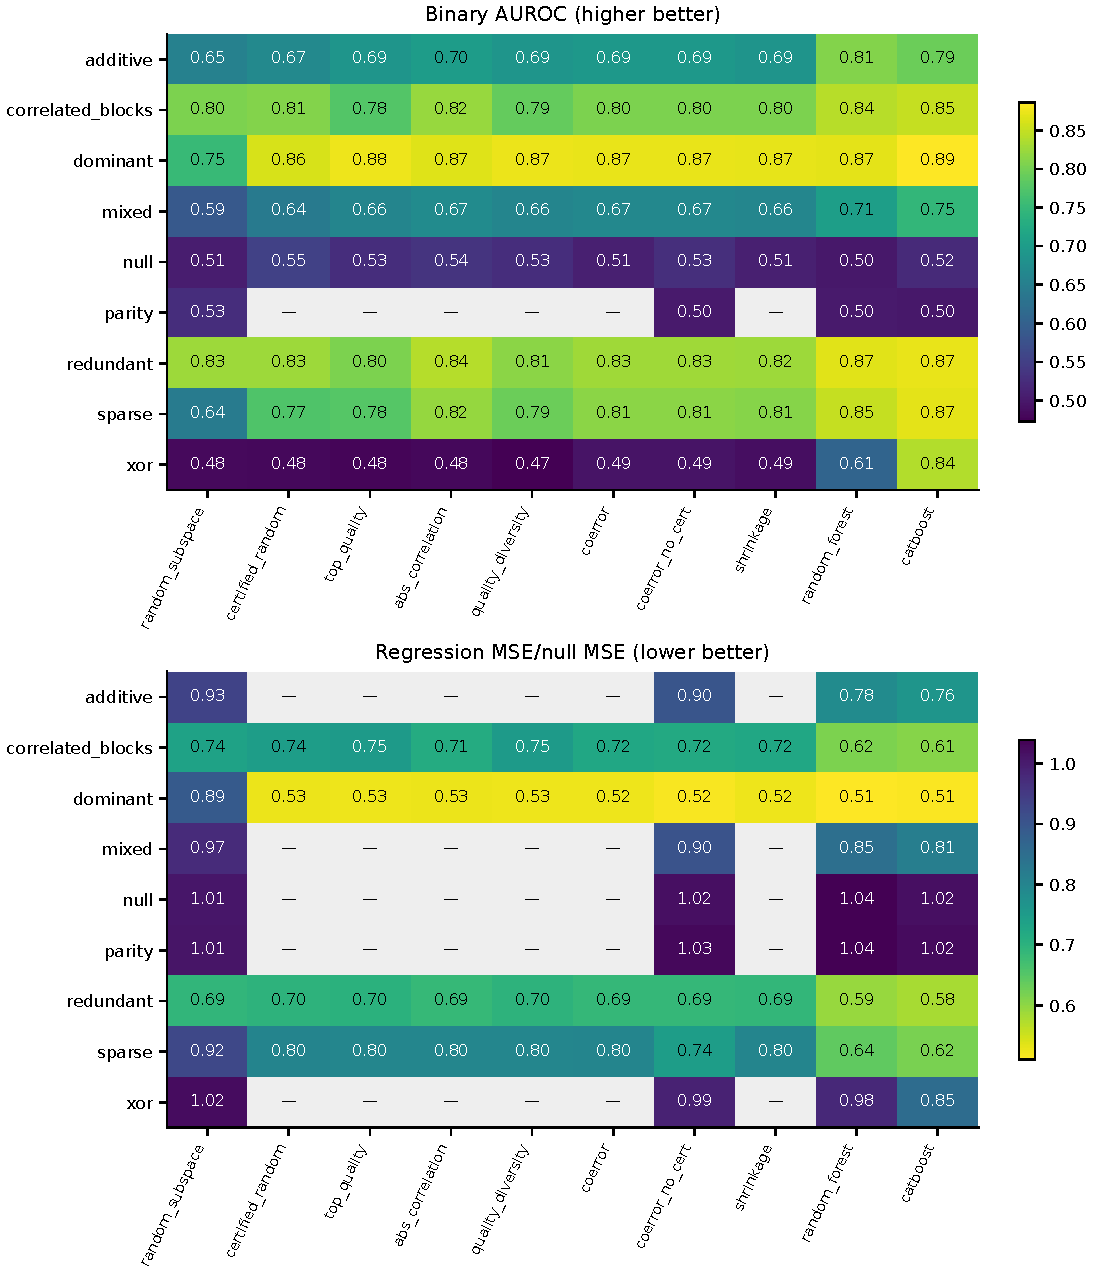
\includegraphics[width=\linewidth]{figures/exp_001_mechanisms_v1/performance.pdf}
\caption{Development mechanism results. Gray cells indicate no feasible fixed-$K$
screened ensemble. Numerical annotations are means of completed splits; the
tables mark partial feasibility. Rankings are not confirmation evidence.}
\end{figure}

The initial hypothesis is not supported as a broad performance claim at these
settings. Unfiltered co-error improves mean binary AUROC over unfiltered top
quality by \ExpOneAucGain{}, but generally trails the strong forests and boosting
models. Co-error does not consistently improve over absolute residual correlation
on outer AUROC or squared loss; a positive aggregate Brier effect is concentrated
in the dominant-feature regime. The $\alpha=0.5$ shrinkage variant fails to improve
on unregularized co-error in the compared task means. These are negative findings
for the preregistered settings, not universal statements about the objectives.

\subsection{Screening Failure and Feasibility}
Screened co-error is feasible in only \ExpOneBinaryFeasible{} of 54 binary splits
and \ExpOneRegressionFeasible{} of 54 regression splits. On every binary null
split, \ExpOneNullMin{}--\ExpOneNullMax{} of 100 candidates pass the empirical
screen, despite population AUROC $0.5$ under this data-generating process.
The bootstrap lower quantile must therefore remain labeled an empirical screen.
Across shared feasible splits, top-quality screening has almost no incremental
benefit over unscreened top quality; it frequently prevents a fixed-size ensemble.

\begin{figure}[t]
\centering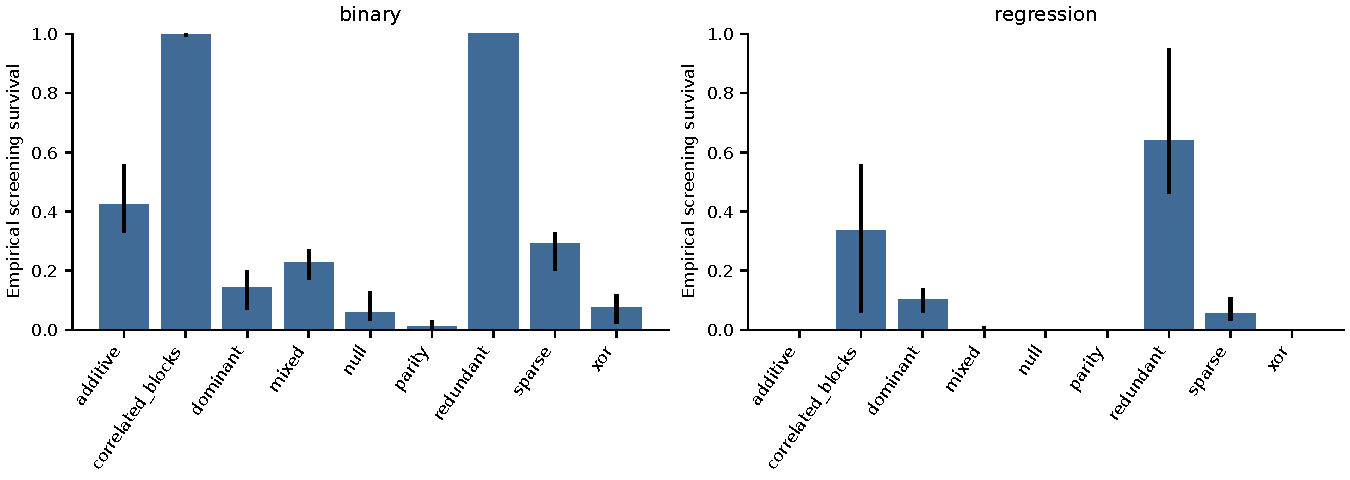
\includegraphics[width=\linewidth]{figures/exp_001_mechanisms_v1/certification.pdf}
\caption{Empirical screening survival by regime. Error bars give the observed
minimum and maximum over folds/seeds, not confidence intervals.}
\end{figure}

\section{Real-World Benchmarks}
No confirmation benchmark has been evaluated. Current benchmark versions and
baseline requirements will be recorded before locking the study.

\section{Ablations and Analysis}
The stored ablations include all required v0 components, signed versus absolute
residual correlation, prediction correlation, covariance without bias, direct
squared-loss greedy selection, with-replacement selection, and shrinkage. An
artifact audit reconstructed loss and test metrics for all selected methods;
the maximum squared-loss/co-error identity discrepancy was below $10^{-12}$.
Direct squared-loss and co-error greedy validation objectives agree, confirming
that their distinction supplies no additional mechanism.

\section{Analysis and Next Discriminating Test}
Additive regression illustrates the attenuation concern: normalized squared loss
is \ExpOneAdditiveCoerror{} for unfiltered co-error, versus
\ExpOneAdditiveForest{} for the unrestricted forest and
\ExpOneAdditiveCatboost{} for CatBoost. This observation does not establish that
attenuation is the sole cause. The next development experiment will compare
the same selected subsets with and without an OOF-fitted aggregate affine
calibrator, then test selection with the affine loss profiled out. Random and
top-quality controls are necessary to determine whether a change comes from
aggregate calibration or a new selection mechanism. Null and dominant-feature
controls will test increased selection/aggregation overfitting.
